\section{Memory Analysis}
\subsection{Memory Overhead}
The memory overhead of our BufferedArrayList implementation consists of two main components:
\begin{itemize}
    \item The array of chunk references: O(n/CHUNK\_SIZE)
    \item The chunk objects themselves: O(n)
\end{itemize}

Therefore, the total memory overhead is bounded by:
\begin{equation}
O(n + \frac{n}{CHUNK\_SIZE})
\end{equation}

\subsection{Memory Efficiency}
For typical chunk sizes (e.g., 64 or 128 elements), the overhead is relatively small:
\begin{itemize}
    \item With CHUNK\_SIZE = 64: overhead $\approx$ 1.56n
    \item With CHUNK\_SIZE = 128: overhead $\approx$ 1.28n
\end{itemize}

\subsection{Memory Access Patterns}
Our implementation exhibits the following memory access characteristics:
\begin{itemize}
    \item Sequential access within chunks
    \item Random access between chunks
    \item Locality-preserving for bulk operations
\end{itemize}

\begin{figure}[t]
\centering
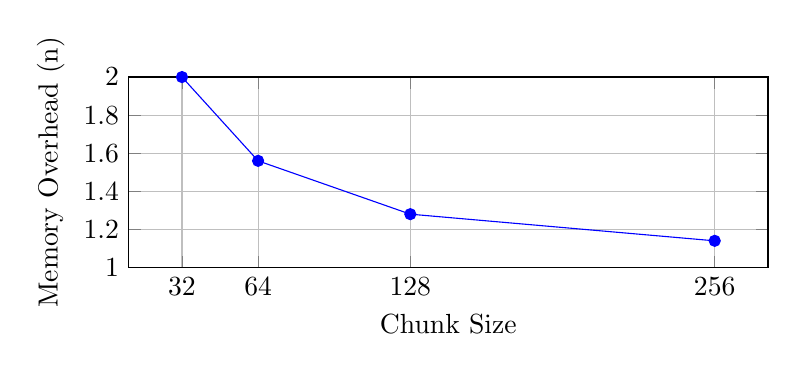
\begin{tikzpicture}
\begin{axis}[
    width=0.8\columnwidth,
    height=4cm,
    xlabel={Chunk Size},
    ylabel={Memory Overhead (n)},
    ymin=1,
    ymax=2,
    xtick={32,64,128,256},
    ytick={1,1.2,1.4,1.6,1.8,2},
    grid=major,
]

\addplot[color=blue,mark=*] coordinates {
    (32,2)
    (64,1.56)
    (128,1.28)
    (256,1.14)
};

\end{axis}
\end{tikzpicture}
\caption{Memory overhead as a function of chunk size}
\label{fig:memory_overhead}
\end{figure} 